% !TEX program = pdflatex
% Overleaf-compatible. Self-contained: only stock packages.
% Compile with pdfLaTeX. Figures live in ./figures/ (generated by
% paper/gen_maps.py and paper/gen_trajectories.py).
\documentclass[11pt]{article}

\usepackage[margin=1in]{geometry}
\usepackage{graphicx}
\usepackage{booktabs}
\usepackage{makecell}
\usepackage{float}
\usepackage{amsmath}
\usepackage{amssymb}
\usepackage{xcolor}
\usepackage{caption}
\usepackage{subcaption}
\usepackage{enumitem}
\usepackage{tikz}
\usetikzlibrary{arrows.meta, positioning, fit, backgrounds, calc}

\captionsetup{font=small, labelfont=bf}

% ---- tile-sprite helper -------------------------------------------------
% \tile{name} renders the 96px composited sprite icon at table-row height.
\newcommand{\tile}[1]{%
  \raisebox{-0.32\height}{\includegraphics[height=2.1em]{figures/tiles/#1.png}}}

% block-diagram node styles
\tikzset{
  blk/.style   = {draw, rounded corners, align=center, font=\small,
                  minimum height=2.6em, fill=blue!8, inner sep=4pt},
  head/.style  = {draw, rounded corners, align=center, font=\small,
                  minimum height=2.4em, fill=orange!14, inner sep=4pt},
  lat/.style   = {draw, rounded corners, align=center, font=\small,
                  minimum height=2.6em, fill=green!10, inner sep=4pt},
  io/.style    = {draw, rounded corners, align=center, font=\small,
                  minimum height=2.6em, fill=gray!10, inner sep=4pt},
  fl/.style    = {-{Stealth[length=2.2mm]}, thick},
}

\title{\textbf{Crafter-in-Cogniland}\\[2pt]
\large A partially-observable navigation env with a one-shot build commitment}
\author{}
\date{}

\begin{document}
\maketitle
\vspace{-2.2em}

\begin{abstract}\noindent
\textsc{Crafter-in-Cogniland} is a small POMDP navigation environment built on
Crafter-style procedural terrain. An agent must cross from a spawn bubble to a
target flag, where the terrain places a \emph{barrier} (a lake or a rocky
ridge) on the direct path. The agent may \textbf{commit once} to building a
\emph{raft} (cancels water slip) or a \emph{harness} (cancels rock slip); the
choice is irreversible and the agent is never told which item it built. The
task therefore couples geometric navigation with a single belief-driven
commitment under partial observation. We train both a recurrent PPO baseline
and a pure-JAX DreamerV3 world model against a shared metric schema.
\end{abstract}

% =======================================================================
\section{Environment at a glance}
% =======================================================================

\begin{description}[leftmargin=1.4em, itemsep=2pt]
\item[Observation] An egocentric tile-id crop plus a few scalars. The two
  trainers consume \emph{slightly different} observations:
  \[
    \underbrace{o_{\text{PPO}} = \{\;\texttt{semantic}_{V\times V},\;
            \texttt{skill\_active}\in\{0,1,2\}\;\}}_{\text{PyTorch env},\ V=21}
    \quad
    \underbrace{o_{\text{Dreamer}} = \{\;\texttt{minimap}_{V\times V},\;
            \texttt{scalars}\in\mathbb{R}^4\;\}}_{\text{JAX env}}.
  \]
  Both crops are the $V{\times}V$ window of tile ids centred on the agent, with
  off-map cells padded by the \texttt{oob} id ($6$). The PPO env's
  \texttt{skill\_active} scalar names \emph{which} item is active
  ($0$=none, $1$=harness, $2$=raft), so the agent need not remember its own
  build. What it \emph{must} still infer is the hidden \emph{map identity}
  (lake vs.\ rocky) --- the local crop never labels the biome.
  Dreamer's \texttt{scalars} additionally supply
  $[\,\text{compass}_r,\ \text{compass}_c,\ \texttt{build\_active},\ t/t_{\max}\,]$:
  a unit vector toward the target and a normalised step counter. PPO receives
  \emph{neither} compass nor step count --- it must read heading from the crop
  alone.
\item[Action] A single discrete action with two terminal build choices:
  \[
    a\in\{\textsf{up},\textsf{down},\textsf{left},\textsf{right},
          \textsf{build\_raft},\textsf{build\_harness}\}.
  \]
  Selecting \textsf{build\_raft} or \textsf{build\_harness} commits that item
  once and for all; later builds are no-ops (still charged a step). The model
  also emits a continuous \texttt{inference\_scalar}$\in[-1,1]$ (the belief
  head, \S\ref{sec:agents}), but that is an internal map-recognition probe,
  \emph{not} an action consumed by the environment.
\item[Reward] Flat slack plus potential-based shaping toward the target:
  \[
    r_t = \underbrace{-0.02}_{\text{slack}}
        \;+\; \underbrace{0.01\,\bigl(\mathrm{ctg}_{t-1}-\mathrm{ctg}_{t}\bigr)}_{\text{PBRS, in cells}},
        \qquad \text{reach bonus } = 0 .
  \]
  $\mathrm{ctg}$ is the unit-cost Dijkstra cost-to-go. With the sparse
  reach bonus disabled, the shaping term is the sole positive signal, so
  returns keep improving as the route tightens (no value cliff at the goal).
\item[Slip] Every tile except \texttt{lava}/\texttt{oob} is walkable. The skill
  is purely a \emph{slip-rate} modifier, and each skill owns \emph{two}
  terrains: \textbf{raft} zeroes \texttt{water} and \texttt{sand}, \textbf{harness}
  zeroes \texttt{dirt} and \texttt{rock}. Stepping onto a tile fails (agent stays
  put) with its base slip unless the matching skill is active: the major
  barriers \texttt{water}/\texttt{rock} slip $0.75$, the minor terrains
  \texttt{sand}/\texttt{dirt} slip $0.30$. \texttt{grass}/\texttt{target} never
  slip; \texttt{tree} always slips $0.75$. So the matching skill clears both its
  barrier \emph{and} the matching apron, while the wrong skill helps neither.
\end{description}

% --------------------------------------------------- tile table
\begin{table}[H]
\centering
\small
\begin{tabular}{clcccp{4.7cm}}
\toprule
\textbf{Sprite} & \textbf{Name} & \textbf{ID} & \textbf{Walkable} &
\textbf{Slip (none\,/\,raft\,/\,harness)} & \textbf{Role} \\
\midrule
\tile{grass}  & \texttt{grass}  & 0 & yes & $0$ / $0$ / $0$ & spawn-bubble \& open ground \\
\tile{dirt}   & \texttt{dirt}   & 1 & yes & $0.30$ / $0.30$ / \textbf{0} & \textbf{harness} apron (rock) \\
\tile{sand}   & \texttt{sand}   & 2 & yes & $0.30$ / \textbf{0} / $0.30$ & \textbf{raft} apron (shoreline) \\
\tile{water}  & \texttt{water}  & 3 & yes & $0.75$ / \textbf{0} / $0.75$ & \textbf{raft} barrier \\
\tile{rock}   & \texttt{rock}   & 4 & yes & $0.75$ / $0.75$ / \textbf{0} & \textbf{harness} barrier \\
\tile{target} & \texttt{target} & 5 & yes & $0$ / $0$ / $0$ & goal cell (flag) \\
\tile{oob}    & \texttt{oob}    & 6 & no  & --- & off-map padding seen in the crop \\
\tile{tree}   & \texttt{tree}   & 7 & yes & $0.75$ / $0.75$ / $0.75$ & always-slips obstacle on grass \\
\tile{lava}   & \texttt{lava}   & 8 & no  & --- & impassable hazard in rock regions \\
\bottomrule
\end{tabular}
\caption{Tile vocabulary and the slip mechanic (slip columns: none\,/\,raft\,/\,harness).
Each skill zeroes \emph{two} terrains (\textbf{bold}): raft $\to$
\texttt{water}+\texttt{sand}, harness $\to$ \texttt{dirt}+\texttt{rock}.
Major barriers slip $0.75$, minor aprons $0.30$; \texttt{grass}/\texttt{target}
never slip.}
\label{tab:tiles}
\end{table}

% =======================================================================
\section{Procedural maps: a compositional generator}
% =======================================================================

Each map is \emph{composed} in three layers rather than thresholded from raw
noise. \textbf{(1) Grass base.} \textbf{(2) Component layer:} a small vocabulary
of analytic terrain \emph{atoms} (Fig.~\ref{fig:components}) --- a bent,
hourglass-thick \emph{ridge} and an irregular \emph{round mountain} (both
\texttt{rock}); a thin meandering \emph{river} and a lobed \emph{lake} (both
\texttt{water}). Each atom is a closed-form field, so placing it is just a
rotation\,$+$\,translation followed by a threshold into a binary mask.
\textbf{(3) Texture layer:} independent simplex fields sprinkle clustered
\texttt{tree} forest and sparse \texttt{dirt}/\texttt{sand} over the open grass,
and a collar of \texttt{dirt} (around ridges) or \texttt{sand} (around water) is
grown a few cells out from each barrier.

The agent travels from a spawn (bottom-left) to a target (top-right), so
barriers are placed to straddle that diagonal --- and the target/spawn keep a
small grass clearance, so a barrier may pass \emph{nearby} the target but never
cover it. The three \textbf{biomes} differ in which atoms appear and how they
are placed:

\begin{itemize}[leftmargin=1.4em, itemsep=1pt]
  \item \textbf{rocky}: a \emph{ridge} with one end pinned to the top-right
        (target) corner, running toward the lower-left, plus a non-overlapping
        \emph{lake}; the ridge wins any overlap $\Rightarrow$ \emph{harness} is the cheap route.
  \item \textbf{lake}: a corner-anchored \emph{river} plus a non-overlapping
        \emph{round mountain}; the river wins any overlap $\Rightarrow$ \emph{raft}.
  \item \textbf{balanced}: the map is split along the anti-diagonal --- one half
        gets a water atom, the other a rock atom, with extra forest down the
        middle grass corridor $\Rightarrow$ building \emph{nothing} is usually best.
\end{itemize}

Because the env is a POMDP, maps are \emph{not} re-sampled to enforce a strict
per-skill cost ordering (as the old simplex pipeline was); the only feasibility
guard is that the target stays reachable.

\begin{figure}[H]
\centering
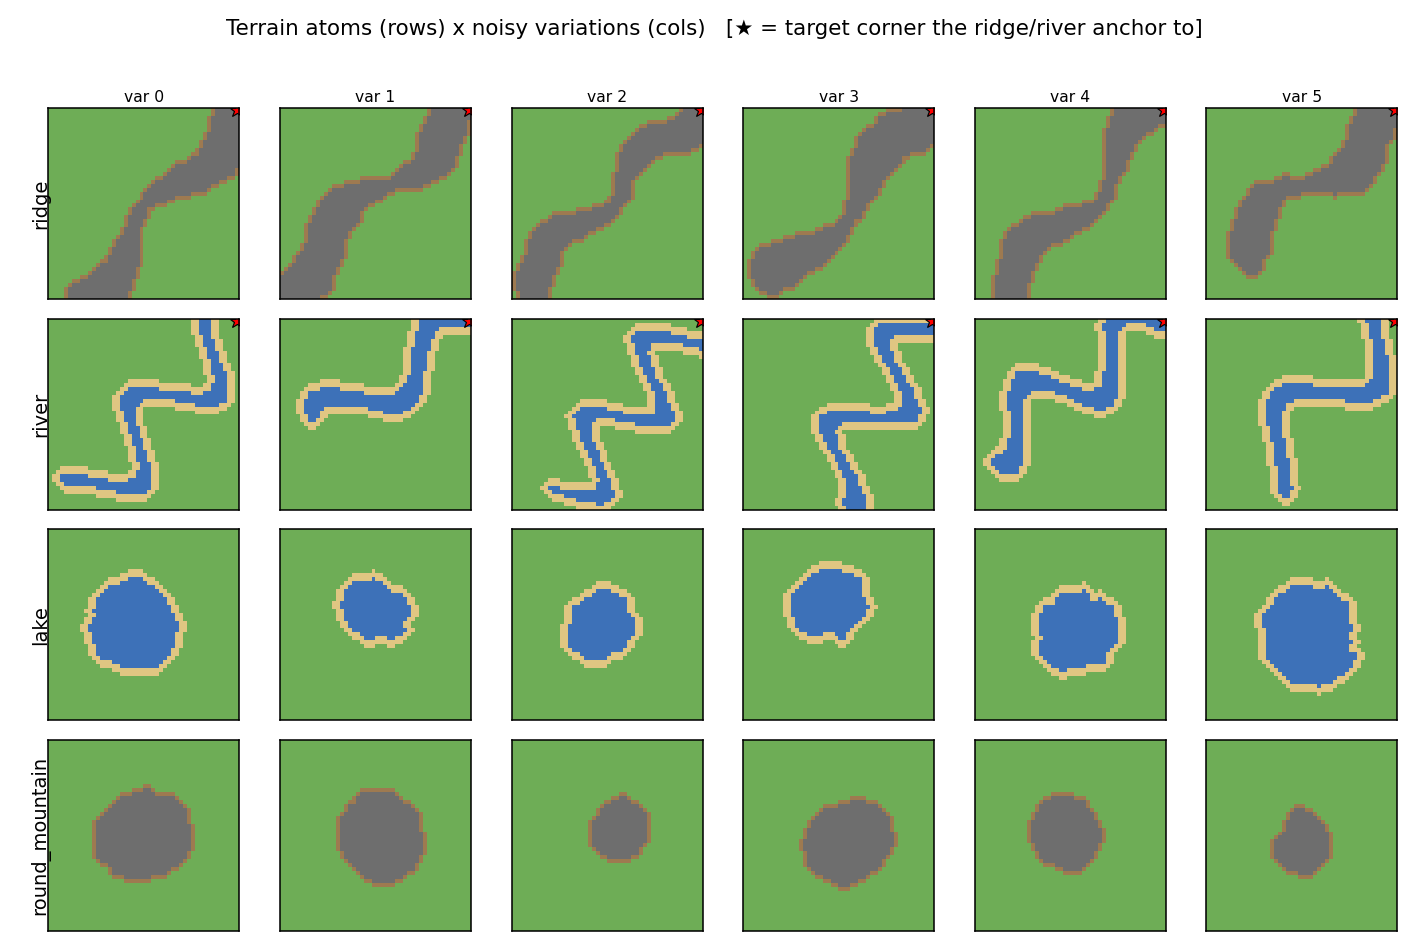
\includegraphics[width=0.92\linewidth]{figures/components_grid.png}
\caption{Terrain atoms (rows) $\times$ noisy variations (columns). Every atom is
an analytic field placed by rotation/translation; \texttt{ridge} and
\texttt{river} are \emph{corner-anchored} --- one end pinned to the target
($\star$) corner --- while \texttt{lake} and \texttt{round\_mountain} are
free-floating blobs. High-frequency simplex noise ragged-ifies each boundary;
water gets a \texttt{sand} beach, rock a \texttt{dirt} skirt.}
\label{fig:components}
\end{figure}

\begin{figure}[H]
\centering
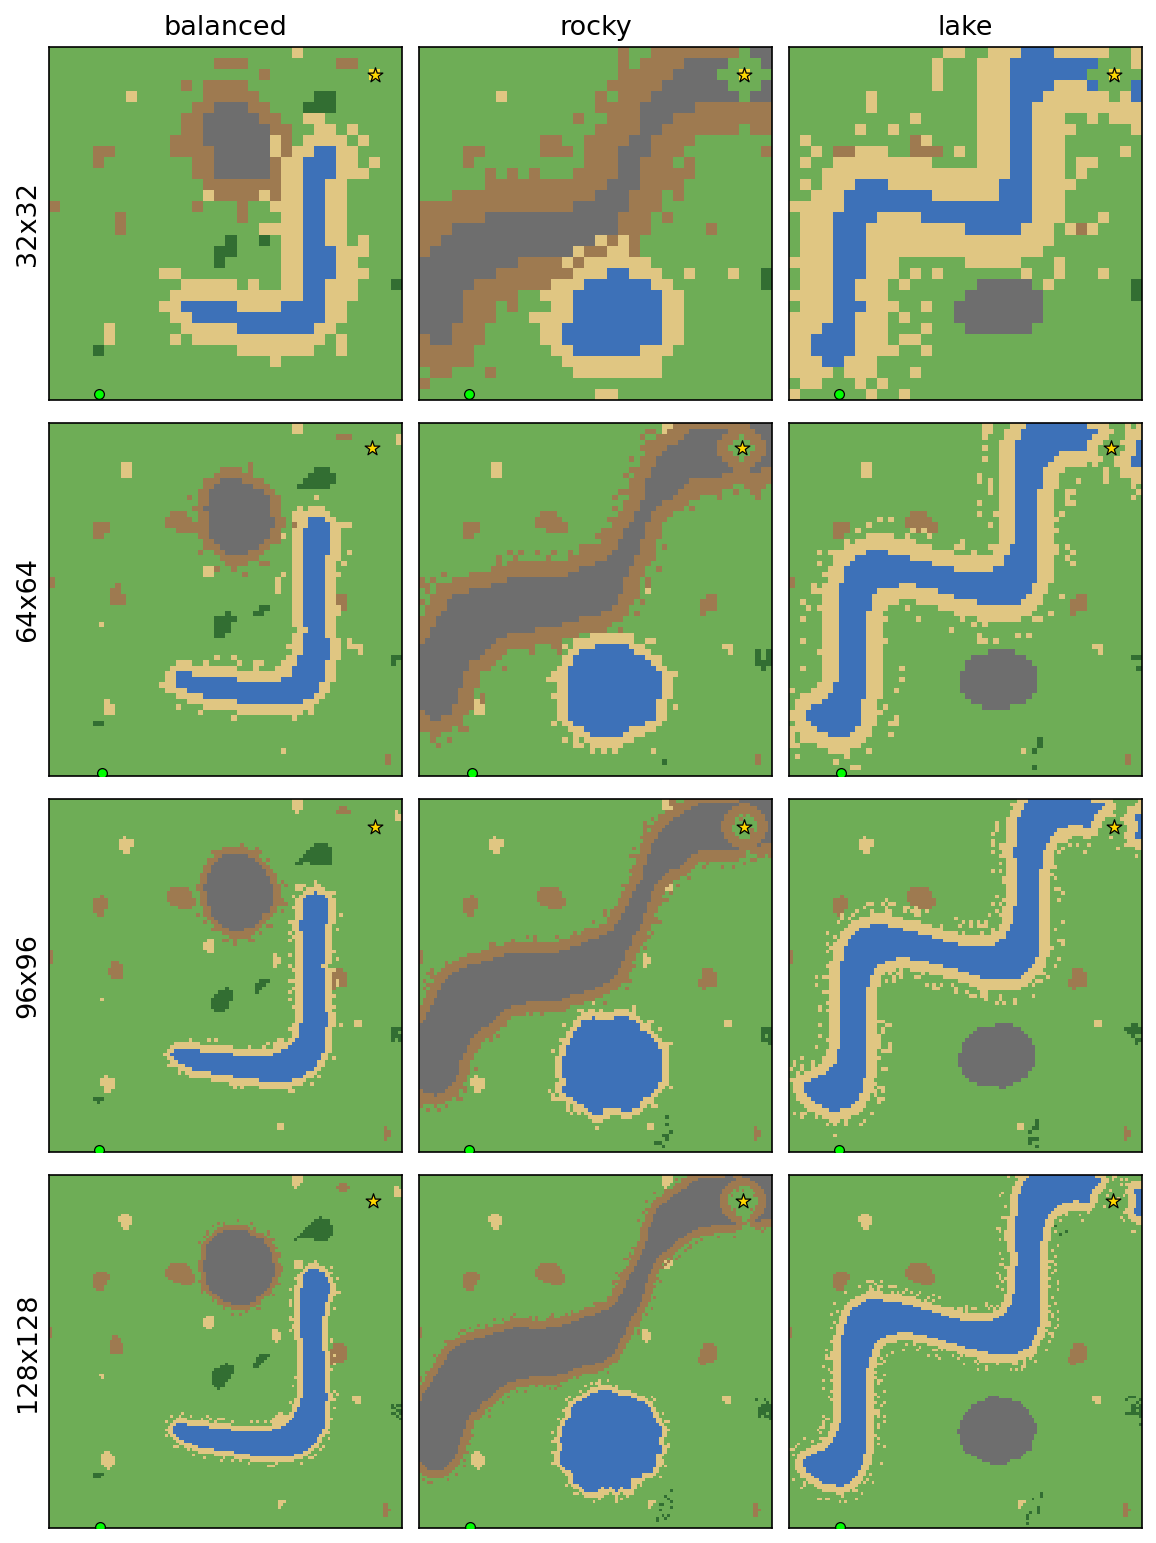
\includegraphics[width=0.62\linewidth]{figures/grid_size_biome.png}
\caption{Map scale $\times$ biome. Rows are side length
($32/64/96/128$); columns are biome (\texttt{balanced}, \texttt{rocky},
\texttt{lake}). Spawn (\textcolor{green!60!black}{$\bullet$}) sits bottom-left,
target (\textcolor{yellow!80!black}{$\star$}) top-right. Blue is \texttt{water},
grey is \texttt{rock}; \texttt{balanced} keeps both scarce.}
\label{fig:sizebiome}
\end{figure}

\begin{figure}[H]
\centering
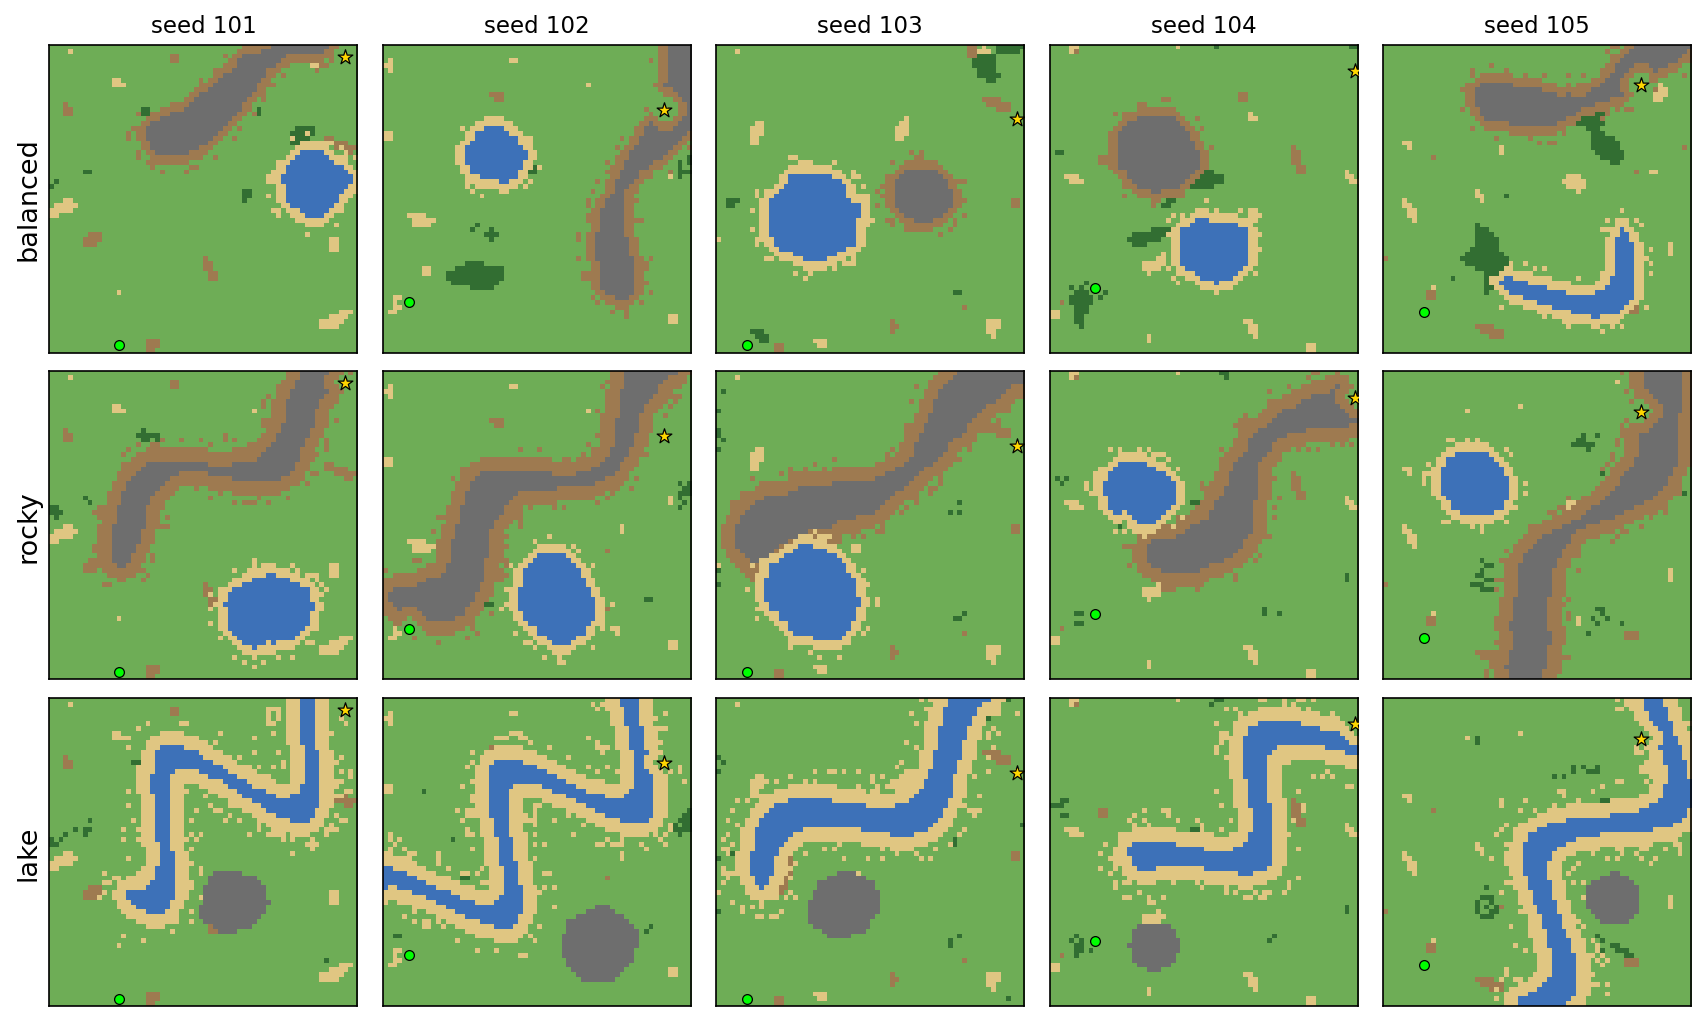
\includegraphics[width=0.92\linewidth]{figures/grid_seeds_64.png}
\caption{Seed diversity at $64\times64$. Rows are biome
(\texttt{balanced}/\texttt{rocky}/\texttt{lake}); columns are different
generation seeds. Each seed yields fresh barrier geometry, so within a biome
the agent cannot memorise a layout --- it must read the local terrain online.}
\label{fig:seeds}
\end{figure}

% =======================================================================
\section{Agents}
\label{sec:agents}
% =======================================================================

\subsection{Recurrent PPO baseline (the released checkpoints)}

The PPO agent is a tile-embedding CNN $\to$ GRU recurrent policy
(Fig.~\ref{fig:ppo}). The $V{\times}V$ tile crop is embedded
($16$-d) and augmented with two CoordConv channels, passed through three
$3{\times}3$ convs, flattened, concatenated with \texttt{skill\_active}, and
projected to a $256$-d embedding. A $128$-unit GRU carries memory across the
episode (so the agent can recall its committed item). Three heads read the GRU
state.

\begin{figure}[H]
\centering
\resizebox{\linewidth}{!}{%
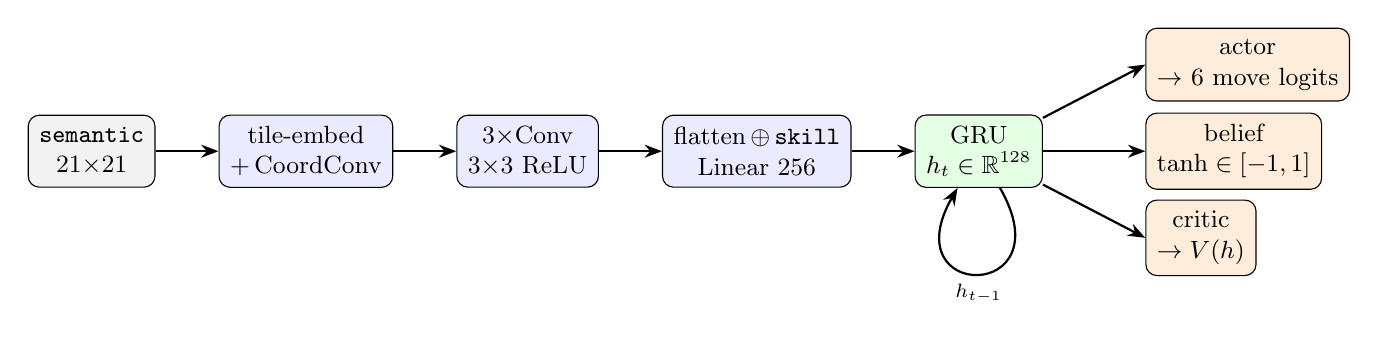
\begin{tikzpicture}[node distance=6mm and 8mm]
  \node[io]  (obs)  {\texttt{semantic}\\$21{\times}21$};
  \node[blk, right=of obs] (emb) {tile-embed\\$+$\,CoordConv};
  \node[blk, right=of emb] (cnn) {$3\times$Conv\\$3{\times}3$ ReLU};
  \node[blk, right=of cnn] (fc)  {flatten\,$\oplus$\,\texttt{skill}\\Linear $256$};
  \node[lat, right=of fc]  (gru) {GRU\\$h_t\in\mathbb{R}^{128}$};
  \node[head, right=13mm of gru, yshift=11mm]  (act) {actor\\$\to$ 6 move logits};
  \node[head, right=13mm of gru]               (bel) {belief\\$\tanh\in[-1,1]$};
  \node[head, right=13mm of gru, yshift=-11mm] (val) {critic\\$\to V(h)$};
  \draw[fl] (obs)--(emb); \draw[fl] (emb)--(cnn); \draw[fl] (cnn)--(fc);
  \draw[fl] (fc)--(gru);
  \draw[fl] (gru)--(act.west); \draw[fl] (gru)--(bel.west); \draw[fl] (gru)--(val.west);
  \draw[fl] (gru) to[out=-60,in=-120,looseness=8]
            node[below,font=\scriptsize]{$h_{t-1}$} (gru);
\end{tikzpicture}}
\caption{PPO-GRU policy. The \emph{belief} head outputs the
\texttt{inference\_scalar}, a deterministic $\tanh$ map-recognition probe; it is
\emph{not} consumed by the env (the build is a discrete action). The actor now
has $6$ move logits (incl.\ \textsf{build\_raft}, \textsf{build\_harness}).}
\label{fig:ppo}
\end{figure}

\paragraph{The inference scalar, and how it is trained.}
The \texttt{inference\_scalar} is produced by the \emph{belief head}: a single
linear unit squashed by $\tanh$ into $[-1,1]$. It is \emph{deterministic}
(unlike the move head, it is not sampled), so $+1$ leans lake/raft, $-1$ leans
rocky/harness, $0$ is undecided. It is \emph{not} an action --- the env never
reads it; the build is committed by the discrete \textsf{build\_raft} /
\textsf{build\_harness} moves instead. The scalar is purely an internal
map-recognition probe that pressures the GRU state to encode the hidden biome.
During training it gets a privileged
\textbf{supervised auxiliary signal}: an MSE loss to the target
$b^\star=\{\textsf{lake}:+1,\ \textsf{rocky}:-1,\ \textsf{balanced}:0\}$ derived
from the map label. The total objective is
\[
  \mathcal{L} = \underbrace{\mathcal{L}^{\text{clip}}_{\text{PPO}}}_{\text{move policy}}
              + 0.5\,\underbrace{\bigl(V-\hat R\bigr)^2}_{\text{value}}
              + 0.5\,\underbrace{\bigl(\tanh(b)-b^\star\bigr)^2}_{\text{belief MSE}}
              - 0.01\,\mathcal{H}[\pi_{\text{move}}].
\]
Each term plays a distinct role, and the gradients are summed because the
four outputs share one trunk (CNN\,$\to$\,GRU) but answer four different
questions:
\begin{itemize}[leftmargin=1.4em, itemsep=1pt]
  \item $\mathcal{L}^{\text{clip}}_{\text{PPO}}$ --- the \textbf{actor} loss. The
        clipped surrogate raises the probability of moves whose advantage
        $\hat A$ is positive while the ratio $\pi/\pi_{\text{old}}$ is clamped to
        $[1{-}0.2,\,1{+}0.2]$, which bounds the policy step per update and keeps
        the on-policy approximation valid. This is the only term that learns
        \emph{where to move}.
  \item $0.5\,(V-\hat R)^2$ --- the \textbf{critic} loss. Regressing the value
        head onto the GAE return $\hat R$ gives the baseline that makes the
        advantage estimate low-variance; without an accurate $V$ the actor's
        $\hat A$ would be noisy and learning would stall. Weight $0.5$ is the
        standard PPO value coefficient.
  \item $0.5\,(\tanh(b)-b^\star)^2$ --- the \textbf{belief} loss. Move reward
        alone teaches the build choice only through a long, noisy credit-
        assignment path (build now $\to$ less slip many steps later). Supervising
        the belief head directly against the privileged label $b^\star$ turns
        \emph{which item to build} into a cheap one-step regression, so the
        commitment is learned reliably; at test time the head still has to infer
        $b$ from the crop, so no privileged information leaks into control.
  \item $-0.01\,\mathcal{H}[\pi_{\text{move}}]$ --- the \textbf{entropy bonus}.
        Subtracting (a small multiple of) the move-policy entropy rewards keeping
        the action distribution spread out, sustaining exploration and stopping
        the policy from collapsing to a deterministic route before it has seen
        enough terrain.
\end{itemize}
Optimiser Adam ($\text{lr}=3\!\times\!10^{-4}$), GAE ($\gamma=0.99$,
$\lambda=0.95$), clip $0.2$, $128$ steps $\times$ $4$ epochs $\times$ $4$
minibatches. The four released checkpoints
(\texttt{ppo\_gru\_size\{32,64,96,128\}}) are each trained for $5\mathrm{M}$ env
steps on \texttt{map\_type=random} at \emph{one fixed map size}.

\subsection{DreamerV3 world model (high level)}

The Dreamer trainer learns a recurrent state-space model (RSSM) and trains the
actor--critic purely \emph{in imagination} (Fig.~\ref{fig:dreamer}). Because the
minimap is symbolic, the encoder/decoder are MLPs (RMSNorm\,+\,SiLU) over the
flat $V{\cdot}V+4$ observation vector (minimap $\oplus$ the 4 scalars) --- no
pixel CNN.

\begin{figure}[H]
\centering
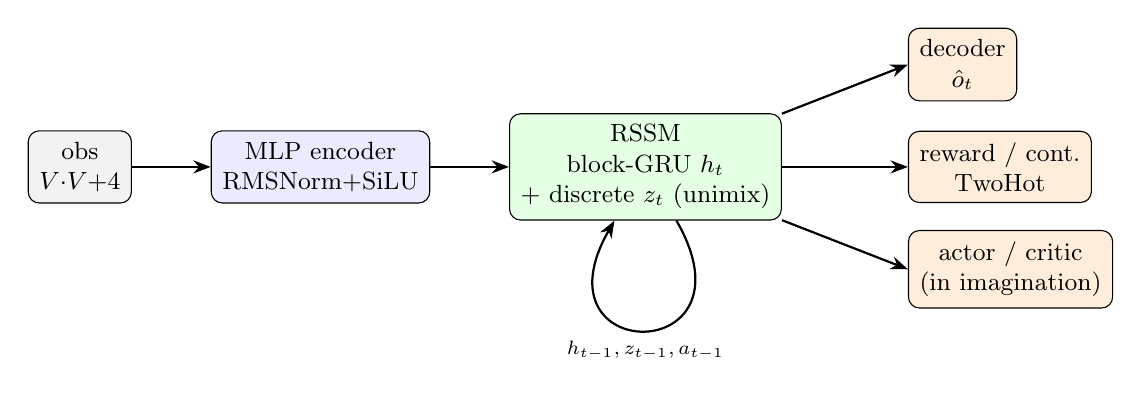
\begin{tikzpicture}[node distance=6mm and 10mm]
  \node[io]  (obs)  {obs\\$V{\cdot}V{+}4$};
  \node[blk, right=of obs] (enc) {MLP encoder\\RMSNorm+SiLU};
  \node[lat, right=of enc] (rssm) {RSSM\\block-GRU $h_t$\\+ discrete $z_t$ (unimix)};
  \node[head, right=16mm of rssm, yshift=13mm] (dec) {decoder\\$\hat o_t$};
  \node[head, right=16mm of rssm, yshift=0mm]  (rew) {reward / cont.\\TwoHot};
  \node[head, right=16mm of rssm, yshift=-13mm](ac)  {actor / critic\\(in imagination)};
  \draw[fl] (obs)--(enc); \draw[fl] (enc)--(rssm);
  \draw[fl] (rssm)--(dec.west); \draw[fl] (rssm)--(rew.west); \draw[fl] (rssm)--(ac.west);
  \draw[fl] (rssm) to[out=-60,in=-120,looseness=7]
            node[below,font=\scriptsize]{$h_{t-1},z_{t-1},a_{t-1}$} (rssm);
\end{tikzpicture}
\caption{High-level DreamerV3. The RSSM rolls forward in latent space; the
actor--critic is optimised on imagined trajectories with $\lambda$-returns and
a slow (EMA) critic.}
\label{fig:dreamer}
\end{figure}

\begin{table}[H]
\centering\small
\begin{tabular}{ll}
\toprule
\textbf{Component} & \textbf{Choice} \\
\midrule
Latent           & deterministic $h$ (block GRU) + discrete stochastic $z$, unimix $1\%$ \\
Reward / value   & TwoHot over $255$ symlog bins \\
Slow critic      & EMA decay $0.98$ + cross-entropy reg \\
Actor scale      & RetNorm $S=\max(1,\mathrm{Per}_{95}-\mathrm{Per}_{5})$ \\
KL loss          & balanced dyn/rep, free-nats $1$, $\beta_{\text{rep}}{=}0.1$ \\
Optimiser        & LaProp ($\varepsilon{=}10^{-20}$) + AGC $0.3$ \\
Defaults         & $\gamma{=}0.997$, $\lambda{=}0.95$, entropy $3{\times}10^{-4}$, lr $4{\times}10^{-5}$ \\
\bottomrule
\end{tabular}
\caption{DreamerV3 components (paper-aligned). The discrete build action folds
the PPO belief scalar into two terminal actions (\textsf{build\_raft},
\textsf{build\_harness}).}
\label{tab:dreamer}
\end{table}

% =======================================================================
\section{Behaviour: 100 stochastic rollouts per map}
% =======================================================================

Figure~\ref{fig:traj} probes each PPO-GRU checkpoint on a \emph{single fixed
map} (identical spawn and target) per biome at the model's trained size. We
sample the move policy $100$ times --- so divergence between paths reflects both
policy stochasticity and terrain slip --- and overlay the trajectories as thin
lines over a darkened map. Crucially, \textbf{each segment is coloured by the
agent's currently-active skill}: dark blue while it carries nothing, orange once
it has built a raft, yellow once it has built a harness. A path that starts blue
and turns orange/yellow part-way thus shows exactly \emph{when} and \emph{what}
the agent committed to.

The bottom row adds the \textbf{skill-choice matrix} (the same quantity logged
to W\&B): for each model, the fraction of the $100$ trials per biome that ended
with each skill (rows \texttt{balanced}/\allowbreak\texttt{rocky}/\allowbreak\texttt{lake},
columns \texttt{noskill}/\allowbreak\texttt{harness}/\allowbreak\texttt{raft}). A competent agent is
near-diagonal: \texttt{lake}$\to$\texttt{raft}, \texttt{rocky}$\to$\texttt{harness},
\texttt{balanced}$\to$\texttt{noskill}.

The full set of grids (both slip regimes, five map seeds each) lives in
\texttt{figures/trajectory\_grids/}; Fig.~\ref{fig:traj} shows the $\text{slip}=0.75$
models on seed $42$. Across seeds the \texttt{lake} and \texttt{rocky} rows
saturate on the correct skill, while \texttt{balanced} stays noisier --- the
hardest case, since the agent must learn to build \emph{nothing}.

\begin{figure}[H]
\centering
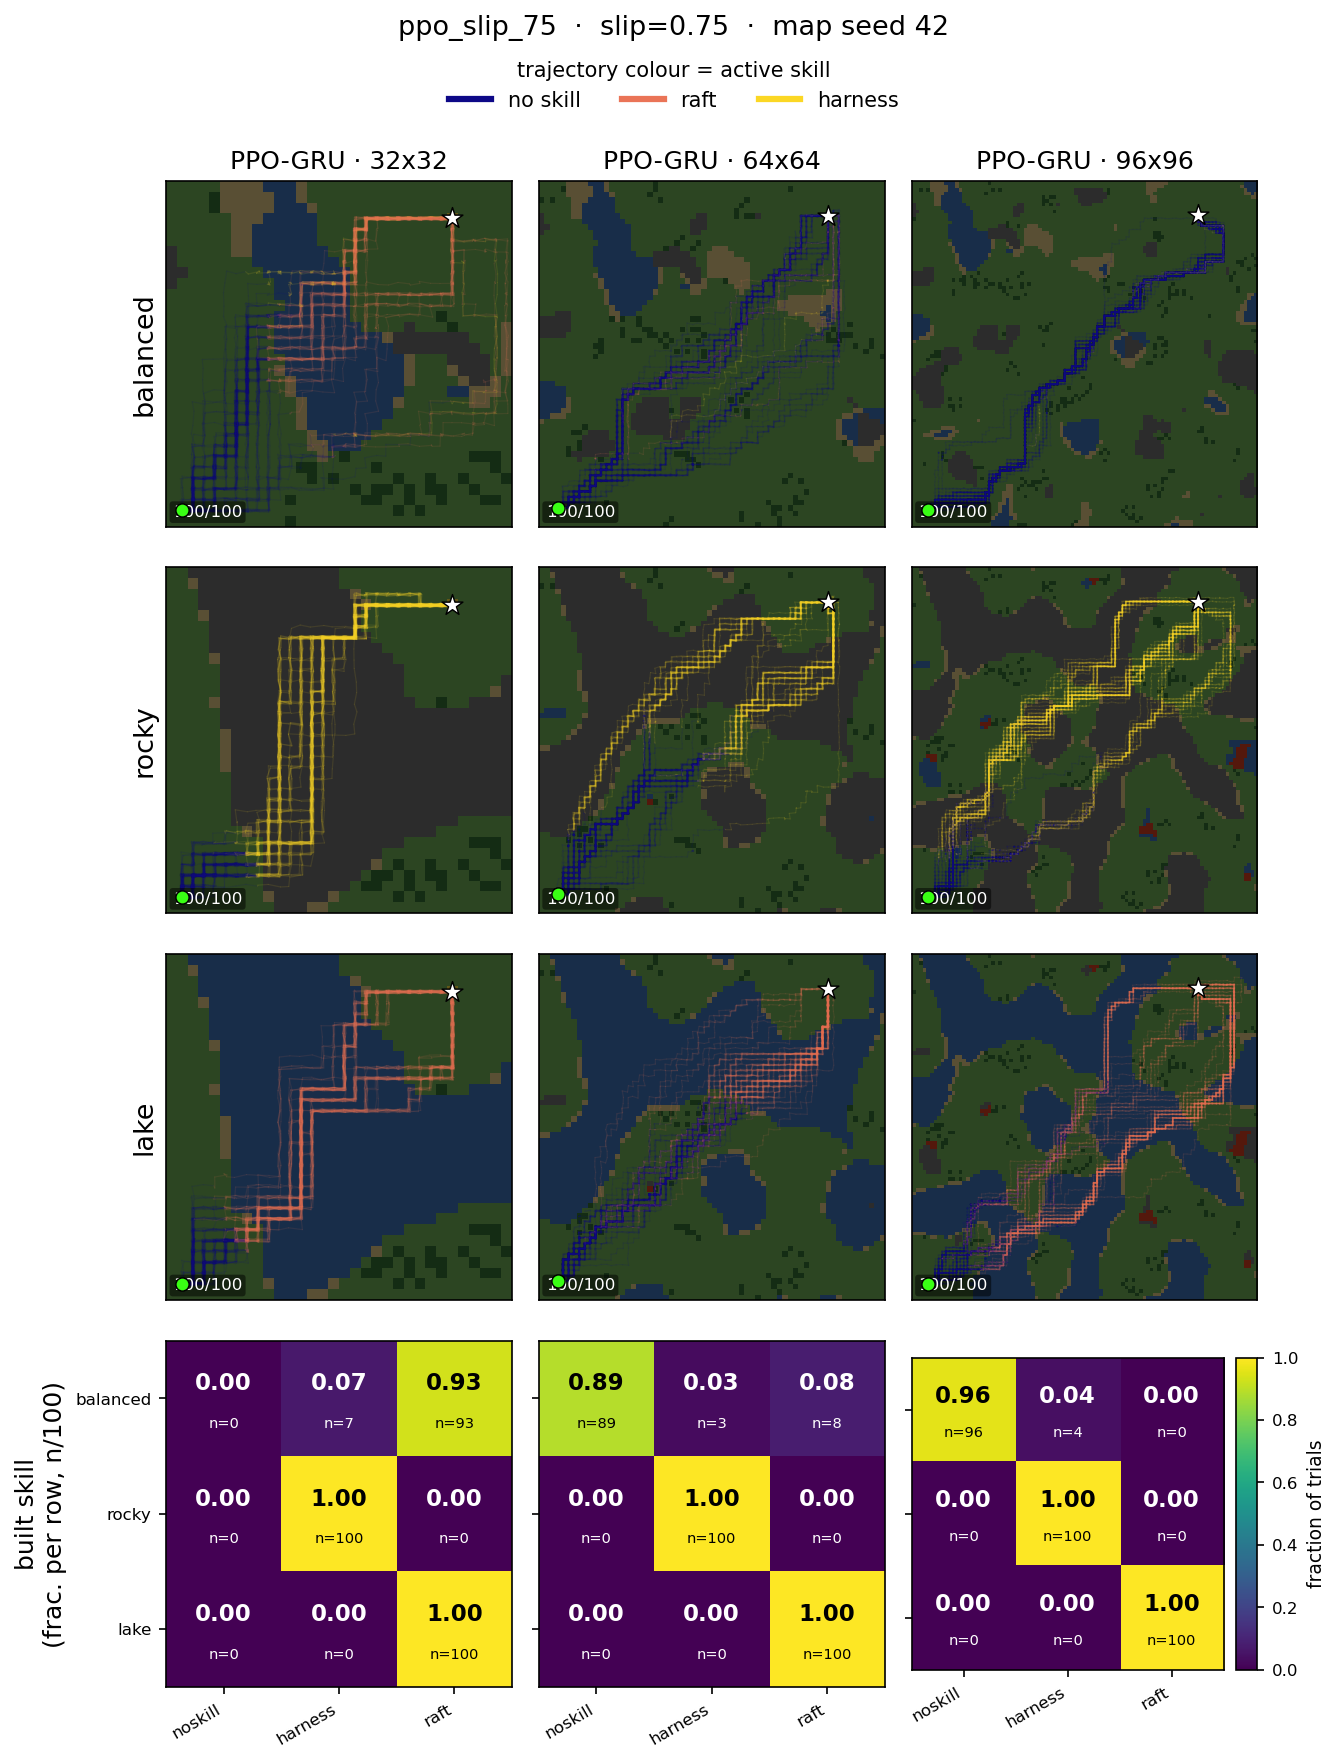
\includegraphics[width=0.80\linewidth]{figures/trajectory_grids/slip_regime/traj_slip75_seed42.png}
\caption{Trajectory + skill grid (\texttt{slip}$=0.75$, map seed $42$). Rows are
biome (\texttt{balanced}/\texttt{rocky}/\texttt{lake}); columns are the PPO-GRU
checkpoint, each on the map size it was trained on (\,$32/64/96$; the $128$ model
is omitted). Trajectory colour = active skill (no skill = dark blue, raft =
orange, harness = yellow); spawn = \textcolor{green!70!black}{$\bullet$},
target = $\star$, inset = successes/$100$. Bottom row: skill-choice matrix,
row-normalised fraction of trials (with raw counts), \texttt{viridis} scale at
right.}
\label{fig:traj}
\end{figure}

\subsection{Measuring path diversity}

To say how \emph{varied} a policy's paths are, we score the $100$ rollouts per
map with two numbers. For each rollout we build its \textbf{occupancy}: the
fraction of steps spent on each map cell (a probability map over cells).

\begin{description}[leftmargin=1.4em, itemsep=3pt]
\item[Occupancy entropy (nats).] Average the $100$ occupancies into one map and
  take its Shannon entropy
  \[
    H = -\sum_{\text{cells } c} p(c)\,\ln p(c)\quad\text{(nats)} .
  \]
  It measures \emph{how much ground is used}: low when every run hugs the same
  short corridor, high when the policy spreads over many cells. Bounded by
  $\ln(\text{visited cells})$.
\item[Across-trajectory JSD (nats).] The Jensen--Shannon divergence among the
  $100$ per-run occupancies,
  \[
    \mathrm{JSD} = H\!\Big(\tfrac{1}{N}\textstyle\sum_i o_i\Big)
                 - \tfrac{1}{N}\textstyle\sum_i H(o_i)\ \ge 0 ,
  \]
  i.e.\ the entropy of the average minus the average entropy. It measures
  \emph{how much the runs differ from each other}: $0$ when all paths are
  identical, larger when each run takes a different route. Bounded by $\ln N$.
\end{description}

The two are complementary: entropy can be high simply because a single wandering
path covers many cells, whereas JSD isolates \emph{between-run} spread. The
\texttt{diverse} preset scores higher on both (occupancy entropy ${\approx}6.5$
nats, JSD ${\approx}2.0$) than the \texttt{efficient} preset (${\approx}5.6$ /
${\approx}1.1$), while both still reach the target --- diversity bought without
giving up the task. Both are computed by
\texttt{cogniland.trajectory\_variability} and logged to W\&B.

\end{document}
